\documentclass[11pt, twoside, a4paper]{article}
\usepackage{color}
\usepackage{tikz}
\usepackage{listings}
\usetikzlibrary{shapes, arrows}
\tikzstyle{decision} = [ diamond, aspect=2, draw, fill=blue!20, text width=5em, text badly centered, node distance=3cm, inner sep=0pt ]
\tikzstyle{block} = [ rectangle, draw, fill=blue!20, text width=5em, text centered, rounded corners, minimum height=4em ]
\tikzstyle{line} = [ draw, -latex' ]
\tikzstyle{cloud} = [draw, ellipse,fill=red!20, node distance=3cm,
    minimum height=2em]


\begin{document}

\title{Bitcoin Zya Service - Worker}
\section {Bitcoin Zya Service - Worker}
\begin{itemize}
  \item Handle Block requests 
  \item Load watch lists 
    \begin{enumerate}
      \item Addresses
      \item Transactions 
    \end{enumerate}
  \item Send status update when done 
  \item Save requests in a database that meet the following conditions.
    \begin{itemize}
      \item
        $(\forall . transactions)
          (to \in addresses \lor from \in addresses \lor tx \in transactions)$
  \end{itemize}
  \item Resume blocks where stopped
  \item Alerts  
\end{itemize}
\section {Node responsibilities}
The purpose of this node is to listen to requests for interacting
a local block (perhaps remote in certain conditions). For example,
querying a block for a set of transactions and publish them.

\section {Commands that the node handles}
\begin {itemize}
  \item QueryBlock for a blockchain (could be bitcoin, ethereum or tezos)
  \item Stop processing the node (a general command that should stop the node)
  \item resume the node.
  \item 
    \begin {itemize}
      \item Add transaction address to a watchlist 
      \item Remove transaction address to a watchlist
      \item Add hash address to a watchlist 
      \item Remove hash address to a watchlist
    \end {itemize}
\end {itemize}
\section {Design}
\begin{lstlisting}[language=Haskell]
module Data.Zya.Bitcoin.Common
...
newtype BlockQuery = 
  BlockQuery { _b :: (BlockHeight, [Address])} deriving (Show, Eq, Generic)

\end{lstlisting}
\section{Block diagram}
\centering
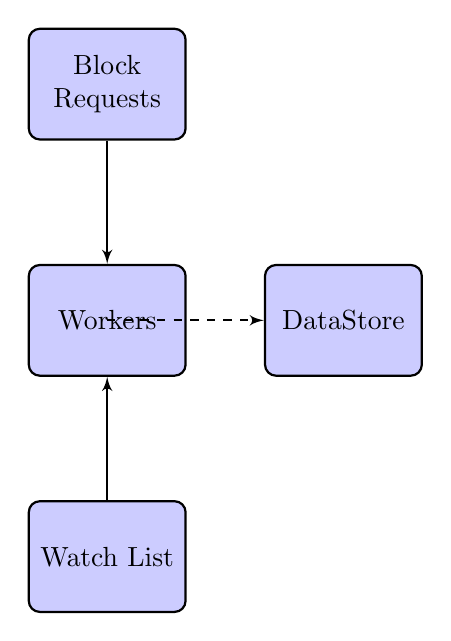
\begin{tikzpicture}[node distance=3cm, auto, scale=1, thick]

% Brief outline
\node [block] (worker)  {Workers};
\node [block, above of = worker ] (requests) {Block Requests};
\node [block, below of= worker] (watchList) {Watch List};
\node [block, right of= worker] (datastore) {DataStore};
\path [line] (requests) -- (worker) ;
\path [line] (watchList) -- (worker) ;
\path [line, dashed] (worker) |- (datastore) ;
\end{tikzpicture}
\end{document}
